\documentclass[12pt]{article}

\usepackage[utf8]{inputenc}
\usepackage[T2A]{fontenc}
\usepackage[english]{babel}
\usepackage{amssymb}
\usepackage{graphicx}
\usepackage{float}
\graphicspath{ {images/} }

\textwidth=431pt
\textheight=600pt
\hoffset=-15pt
\voffset=-15pt

\usepackage{graphicx}
\usepackage{amsmath}
\makeatletter
\renewcommand{\@oddhead}{%
\vbox{%
\hbox to \textwidth{\strut \textit{CV, Assignment 4, Usvyatsov Mikhail} \hfill }
\hrule
\vspace{12pt}
}}
\renewcommand{\@oddfoot}{}
\makeatother

\begin{document}
	\bigskip
	\textbf{Algorithm}
	
For every video for every frame :\\
	\begin{enumerate}
		\item Clear the noise from frame with Gaussian filter;
		\item Extract Background;
		\item Clear the noise from background;
		\item Find contours on background;
		\item Filter small contours with sides greater than MIN\_RECT\_SIZE;
		\item Compare contours from previous frame with contours on current frame;
		\item if there are intersected frames of almost equal size ( difference in SIZE\_CHANGE times) on different frames, than we increase Time To Live (TTL) for them and store the contours from the last frame with current TTL;
		\item If current TTL reach TTL\_THRESHOLD then new object is on the scene for a long time;
		\item If the object with big TTL was lost on the current frame, we put it to the temporary storage;
		\item If it is not found for 5 frames than delete this contours and report it;
	\end{enumerate}
	
	Here are a few results of image processing:\\
	
	\begin{figure}[H]
		\centering
		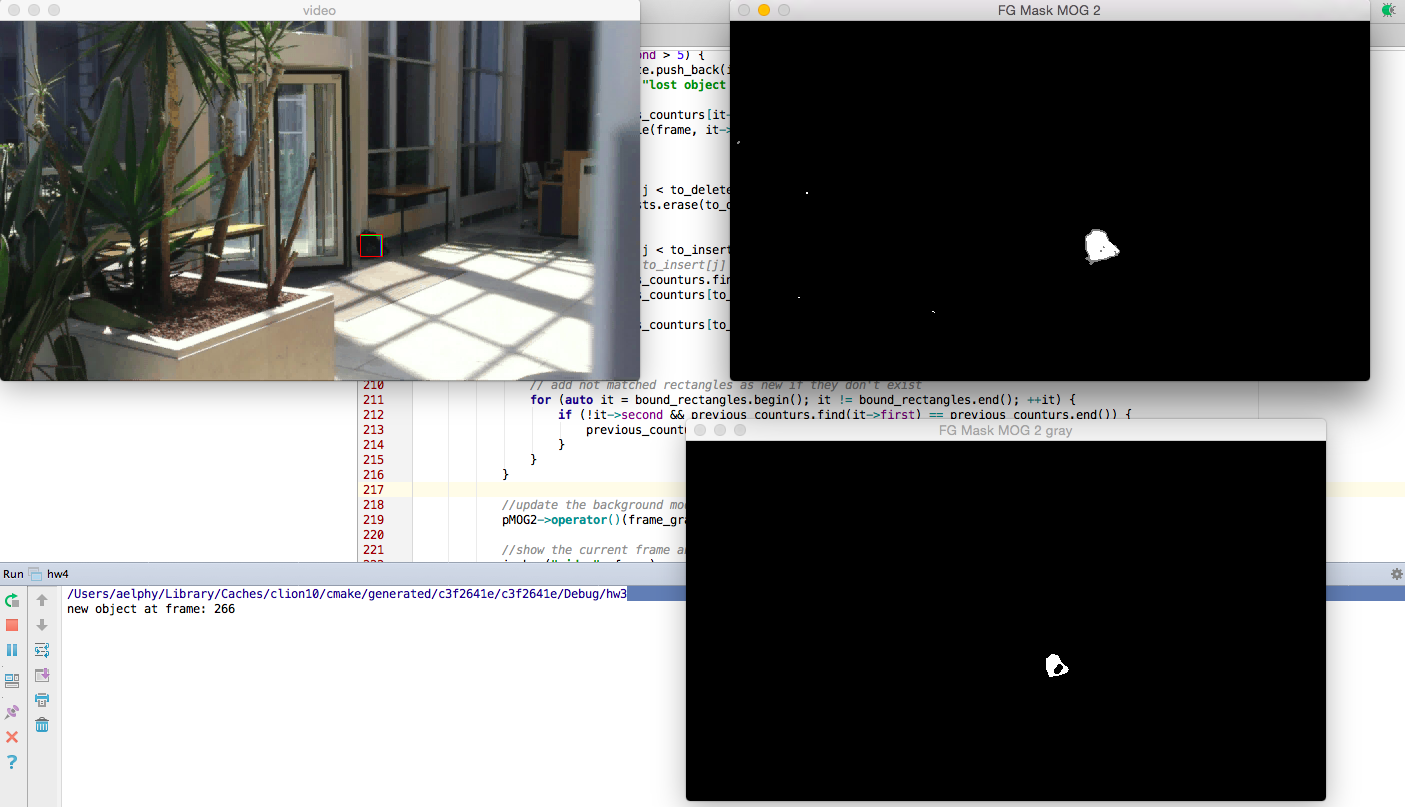
\includegraphics[width=15cm]{1}
		\caption{"Left thing was recognised"}
	\end{figure}
	
	\begin{figure}[H]
		\centering
		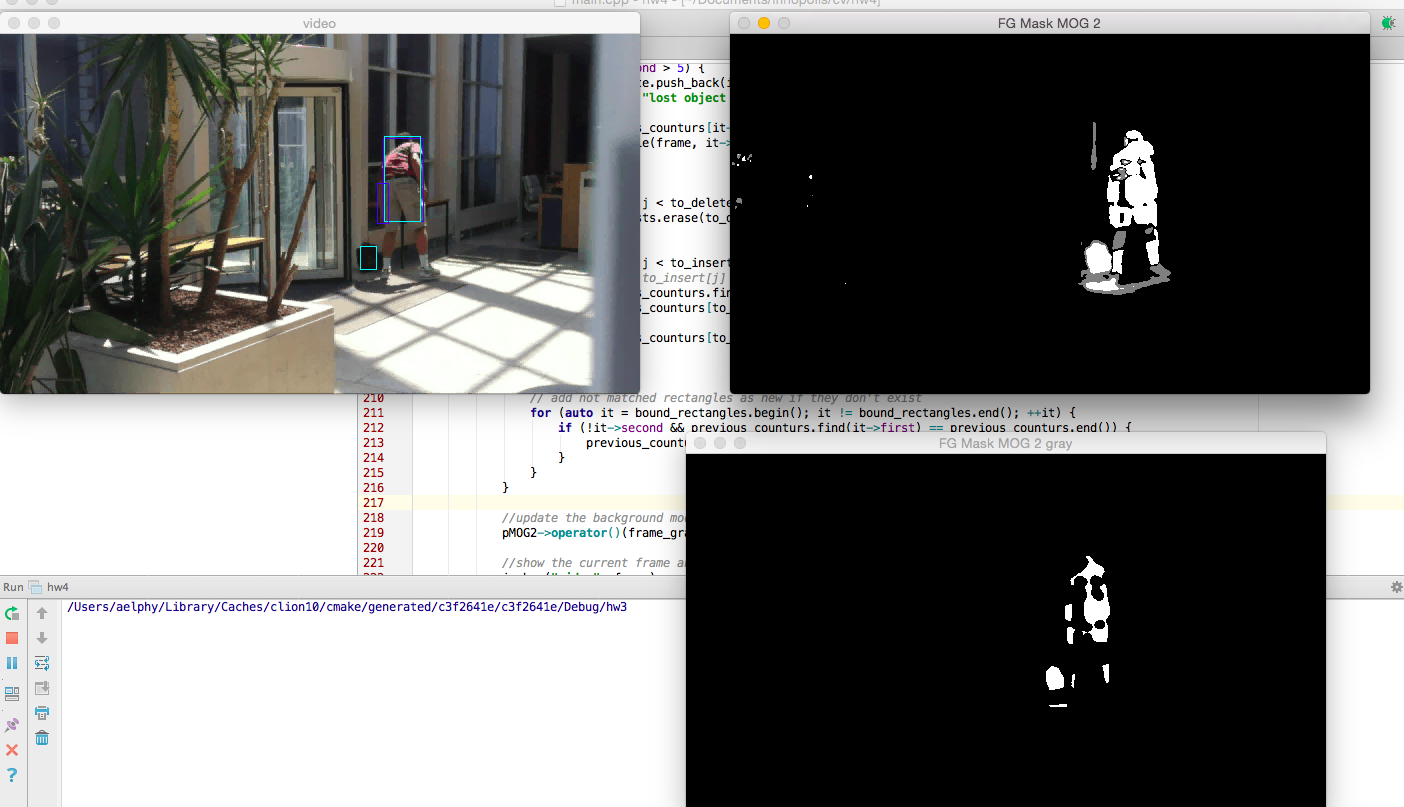
\includegraphics[width=15cm]{2}
		\caption{"Left thing is not yet recognised"}
	\end{figure}
	
	\medskip
	
	\textbf{Results}
	
	The results of the program:

	video 1\\
	new object at frame: 266
	lost object at frame: 403

	video 2\\
	new object at frame: 224
	new object at frame: 240
	lost object at frame: 409
	lost object at frame: 429
	
	two objects on video two are because of the light divided backpack into two visual parts.
	
\end{document}